\documentclass{standalone}
\usepackage{tikz}
\usepackage{ctex,siunitx}
\usepackage{tkz-euclide}
\usepackage{amsmath}
\usetikzlibrary{patterns, calc}
\usetikzlibrary {decorations.pathmorphing, decorations.pathreplacing, decorations.shapes,}
\begin{document}
\small
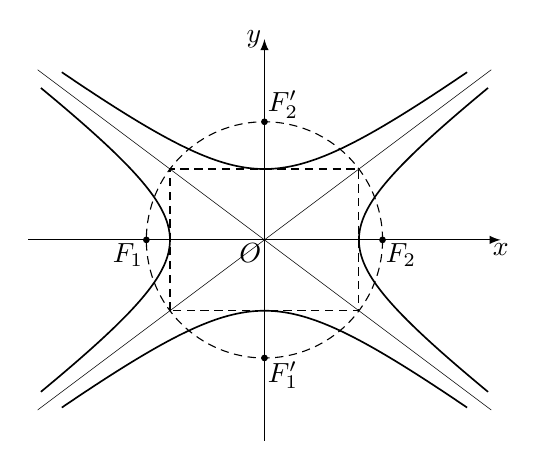
\begin{tikzpicture}[>=latex,scale=1.5,inner sep=1pt]
  \draw[thin,->](-2,0)--(2,0)node[below]{$x$};
  \draw[thin,->](0,-1.7)--(0,1.7)node[left]{$y$};
  \tkzDefPoints{0/0/O,-1/0/F1,1/0/F2,0/-1/F3,0/1/F4,-0.8/-0.6/A,0.8/0.6/B,0.8/-0.6/C,-0.8/0.6/D}
  \draw[semithick,domain=-65:65,samples=200] plot ({0.8/cos(\x)},{0.6*tan(\x)});
  \draw[semithick,domain=-65:65,samples=200] plot ({0.8*tan(\x)},{0.6/cos(\x)});
  \draw[semithick,domain=-65:65,samples=200] plot ({-0.8/cos(\x)},{0.6*tan(\x)});
  \draw[semithick,domain=-65:65,samples=200] plot ({0.8*tan(\x)},{-0.6/cos(\x)});
  \draw[densely dashed](-0.8,-0.6)rectangle(0.8,0.6);
  \draw[densely dashed](0,0)circle(1);
  \tkzDrawPoints[fill=black](F1,F2,F3,F4)
  \tkzLabelPoint[below left](F1){$F_1$}
  \tkzLabelPoint[below right](F2){$F_2$}
  \tkzLabelPoint[below right](F3){$F'_1$}
  \tkzLabelPoint[above right](F4){$F'_2$}
  \tkzDrawLine[add=0.7 and 0.7](A,B)
  \tkzDrawLine[add=0.7 and 0.7](C,D)
  \tkzLabelPoints[below left](O)
\end{tikzpicture}
\end{document}